\chapter{Introduction}
\begin{refsection}
\section{Genomic Dark Matter}
\noindent For most of human history, the microbial world has not been more than ideas and imagination. That was until the late 17th century, when Antonie van Leeuwenhoek, a Dutch microscopist, was the first person to see microbes due to his exceptional skill in making single-lens microscopes~\citep{van1665observations,asimov1972asimov,lane2015unseen}. But it wasn't until the 19th century that Christian Gottfried Ehrenberg coined the word \textit{Bacterium} in 1828~\citep{ehrenberg1828symbolae} and Louis Pasteur disproved the theory of spontaneous generation~\citep{pasteur1862memoire}, the thought that life can commonly arise from non-living matter, and the study of bacteria became of broader interest. For the last two centuries, scientists from various backgrounds have studied the smallest forms of life as we know it, and yet, to date, we have not solved a single organism to the level where we know what every component in a cell is doing and how they are all connected. Even in the case of \textit{Escherichia coli}, a bacterium discovered by Theodor Escherich in 1885~\citep{escherich1885darmbacterien}, arguably the most studied prokaryotic model organism since the isolation of its K12 strain in 1922~\citep{bachmann1972pedigrees}, large parts of its fundamental biology remain a mystery.

\indent Since the characterization of beta-D-galactosidase in 1950~\citep{lederberg1950beta}, the function of many genes in \textit{E. coli} K12 has been annotated. When its genome was fully sequenced for the first time in 1997, 4288 protein-coding open reading frames were identified~\citep{blattner1997complete} and genes were labeled by proposed function. Genes for which no function could be proposed either by previous work or by homology to genes with known function in other organisms were labeled with a \textit{y} as the first letter. However, after 75 years of work, about one-third of \textit{E. coli}'s protein-coding sequences remain without functional annotation, a group of genes that has been coined the \textit{y-ome}~\citep{ghatak2019ome,moore2024revisiting}. In a 2016 study, the concentration of all proteins in \textit{E. coli} cells was measured in 22 different growth conditions. While the resulting data set is incredibly rich and powerful, it also shows that only about 58\% of genes account for more than 95\% of the protein mass in a cell.
\begin{figure}[hbt!]
\centering
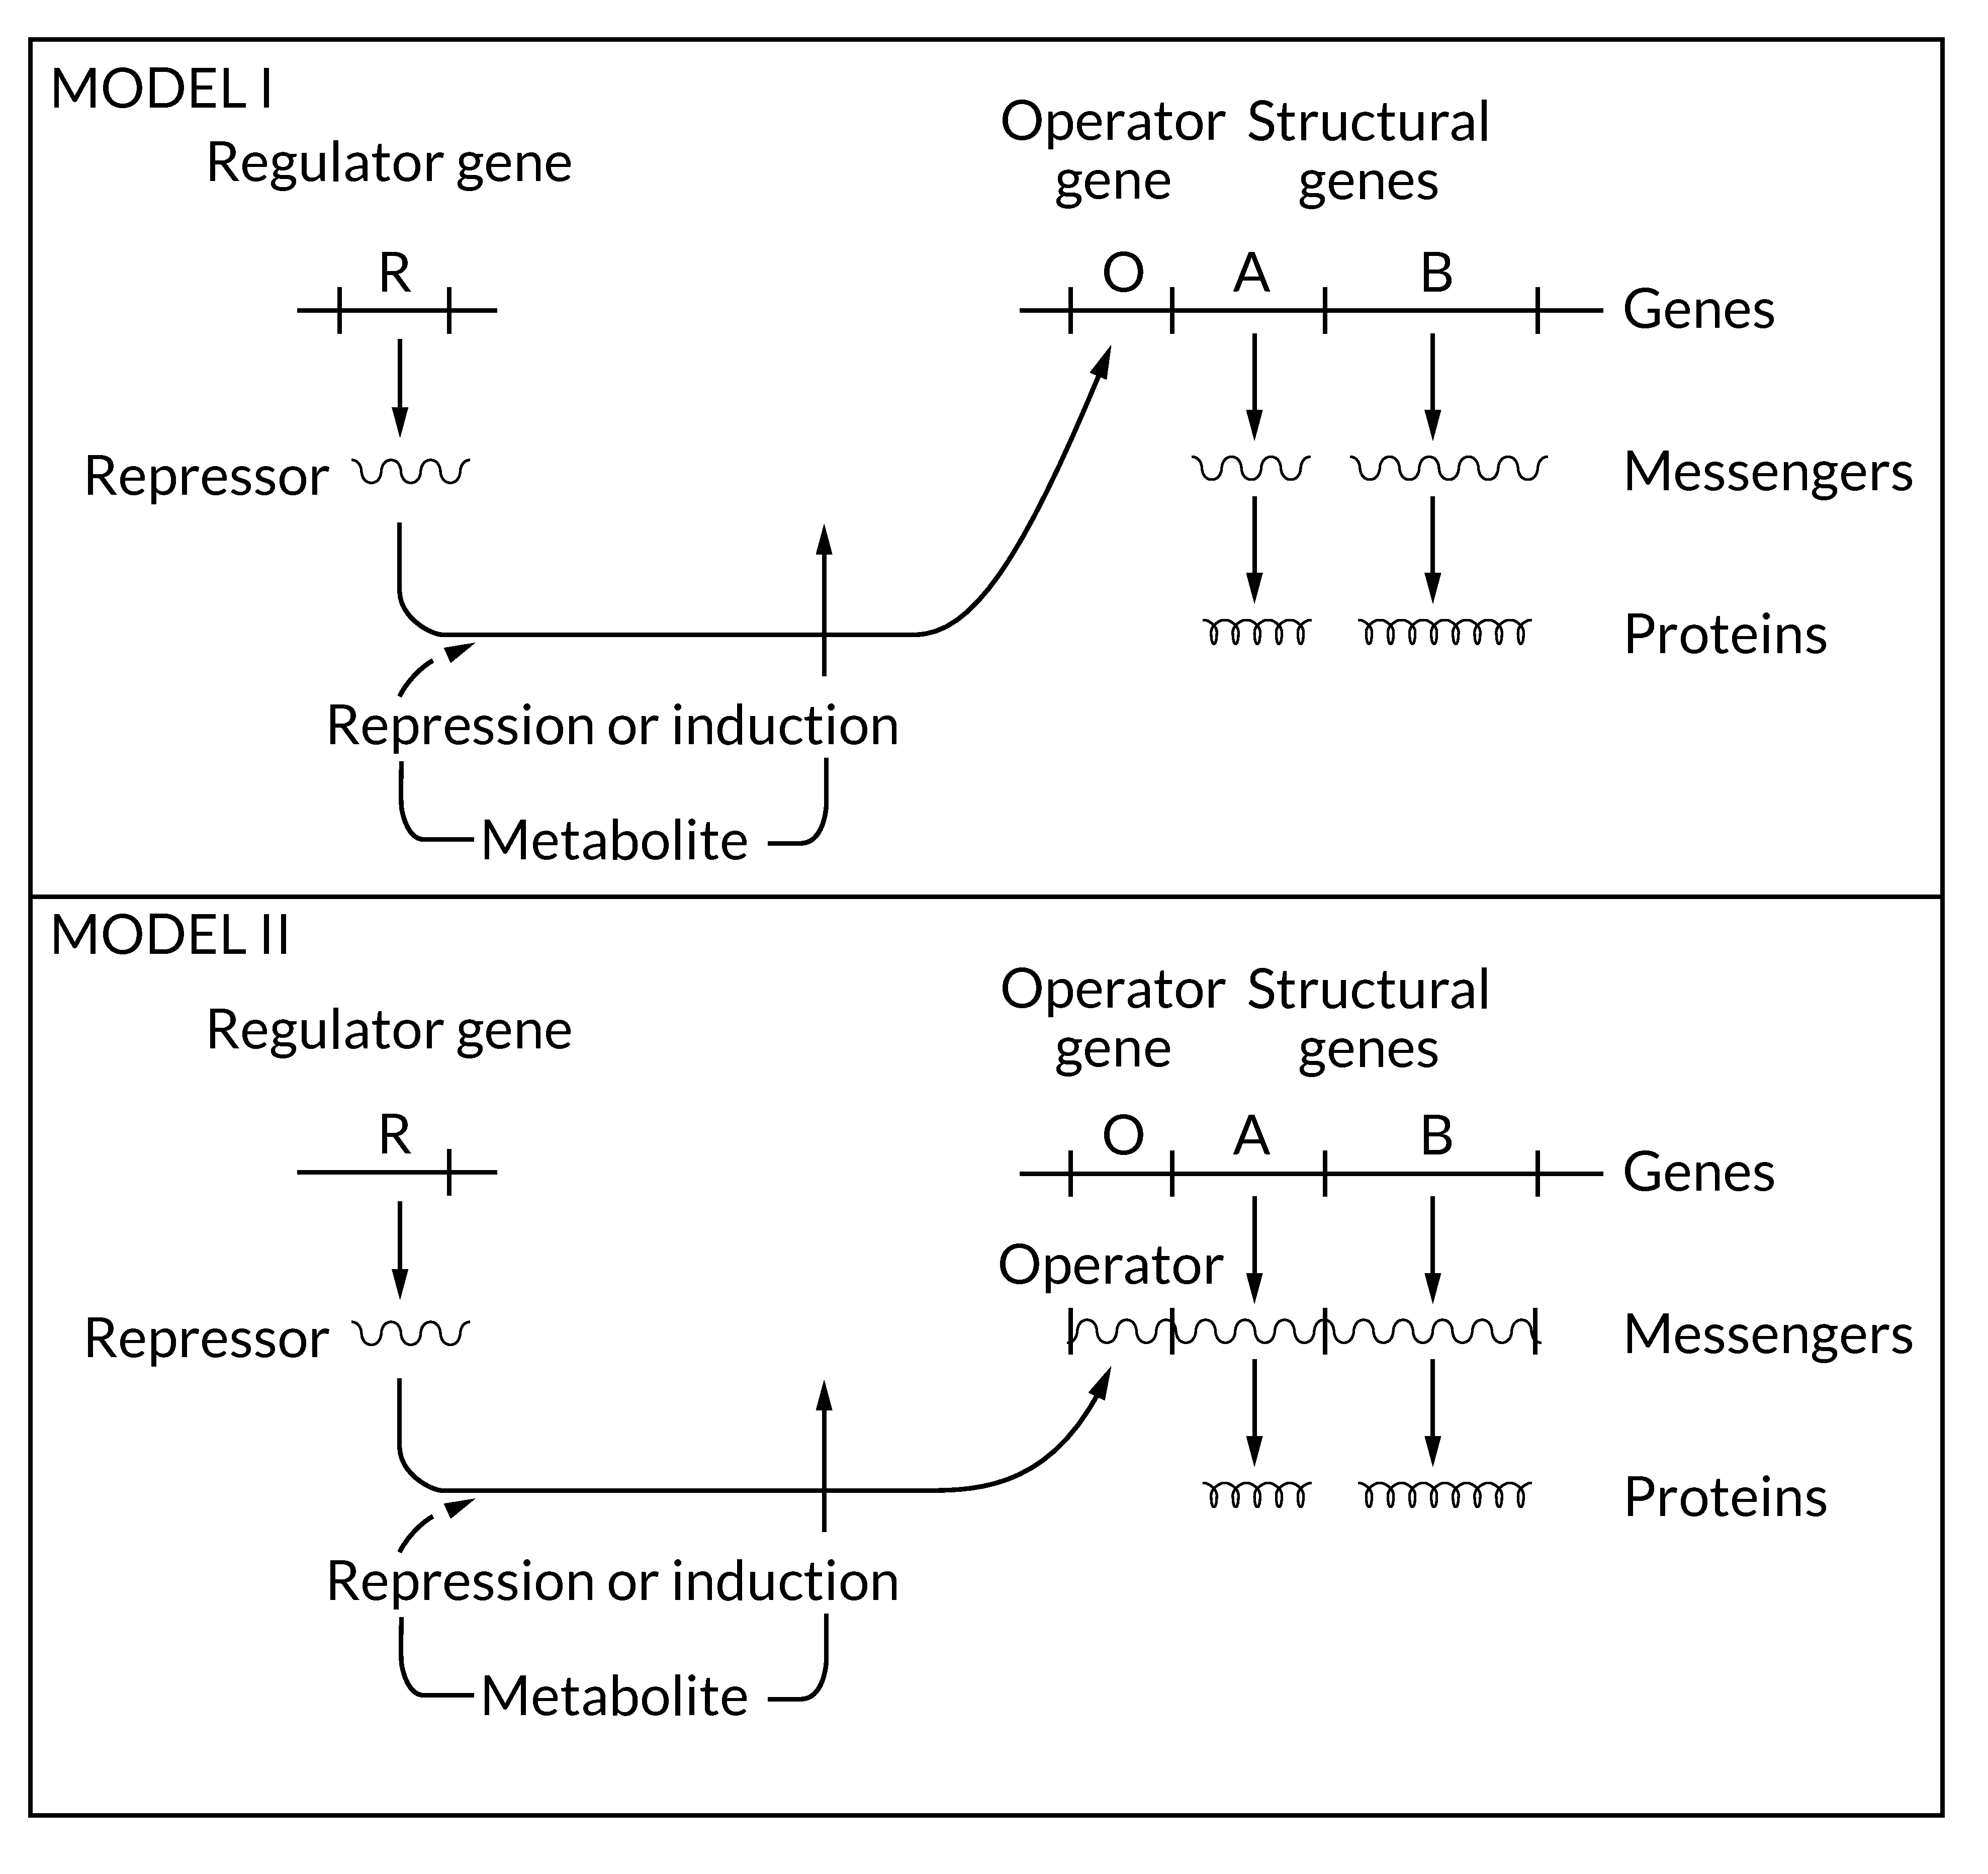
\includegraphics[width=.7\textwidth]{figures/Jacob_Monod_fig6.pdf}
\caption[Discovery of gene regulation by Jacob and Monod.]{\textbf{Discovery of gene regulation.} The two models of gene regulation in the lac-operon proposed by Jacob and Monod, the genetic operator model (Model 1) and the cytoplasmic operator model (Model 2). Schematic recreated from Jacob's and Monod's paper~\citep{jacob1961genetic}.}\label{fig:jacob_monod}
\index{figures}
\end{figure}\\
\indent In addition to identifying a gene's function, it is equally important to know when the gene is expressed. Fran{\c{c}}ois Jacob and Jacques Monod famously discovered the mechanism of repression and inducible expression of the lac-operon in 1961~\citep{jacob1961genetic}. While this work contains many more fundamental discoveries, such as the prediction of mRNA and its short lifetime and the disproval of the \textit{one gene, one enzyme} hypothesis, we focus on the discovery of the \textit{operon}. They found that a protein encoded in a different genomic location can control the expression of a set of genes by interacting with a piece of DNA. As shown in Figure~\ref{fig:jacob_monod}, Jacob and Monod discussed two possible models of repression, which they coined the "genetic operator model" (Model 1) and the "cytoplasmic operator model" (Model 2). In the genetic operator model, the repressor-operator interaction occurs at the genetic level, with the repressor directly controlling the synthesis of the gene. By considering the kinetics implied from this model, that the lifetime of the messenger molecule is short and that synthesis of the target gene should be stopped immediately once the gene is removed from the cell, this model was identified as the most likely. And as we know now, the lac repressor binds to DNA, inhibiting expression from the promoter of the lac operon by both sterically blocking binding of the RNA polymerase and by DNA looping, and the lifetimes of mRNA are on the order of minutes \\
In the cytoplasmic operator model, the repressor binds to the messenger RNA, regulating its translation into protein. Jacob and Monod conclude that this model is unlikely because the size of RNA molecules it would require does not agree with the distributions of mRNA sizes measured at the time. Also, this model would require the messenger molecule to have much longer lifetimes. Jacob and Monod specifically noted that they could not disprove this model, and now we know that parts of it exist as small RNAs that can inhibit translation of mRNAs. It should also be noted that at the time of this work, neither the ribosome nor RNA polymerase had been discovered, which makes the discoveries and predictions Jacob and Monod proposed even more impressive.\\
\indent In the decades since Jacob's and Monod's monumental work, the study of gene regulation in prokaryotes has advanced significantly. As will be explained below, it is fair to say that we both know a lot and at the same time very little about how genes are regulated in bacteria.
\begin{figure}[hbt!]
\centering
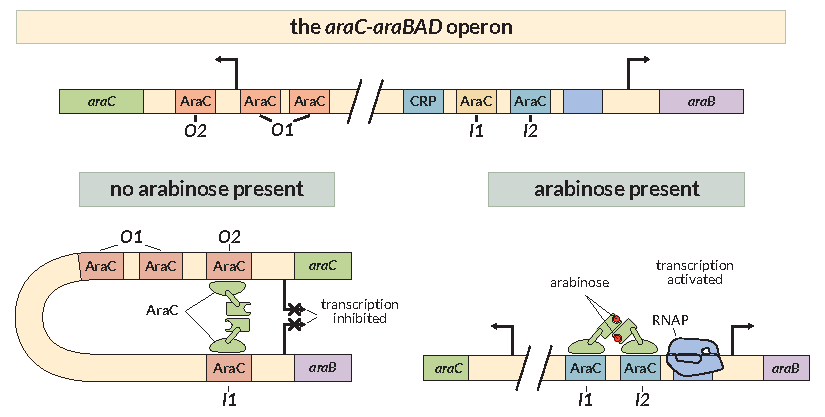
\includegraphics[width=\textwidth]{figures/araB_operon_annotation.pdf}
\caption[Gene Regulation of the \textit{araC}-\textit{araBAD} operon.]{\textbf{Gene Regulation of the \textit{araC}-\textit{araBAD} operon.}}\label{fig:araBAD}
\index{figures}
\end{figure}\\ 
One of the best studied operons in \textit{E. coli} is the ara-operon, which was investigated in excruciating detail by the lab of Robert Schleif. This operon is responsible for the metabolism of L-arabinose and consists of the genes \textit{araBAD} and its divergently expressed regulator \textit{araC}~\citep{greenblatt1971arabinose}. As shown in Figure~\ref{fig:araBAD}, it was discovered that in the absence of L-arabinose, AraC forms a dimer out of two homodimers and binds to two distant binding sites (\textit{I1} and \textit{O2}), leading to the formation of a DNA loop, which suppresses expression from the promoters for \textit{araC} and \textit{araBAD}~\citep{dunn1984operator,martin1986dna,lobell1990dna}. If L-arabinose is present, it binds to each AraC dimer, leading to a conformational change and binding of the complex to the \textit{I1} and \textit{I2} binding sites in the \textit{araBAD} promoter. In this configuration, AraC initiates transcription, and arabinose is metabolised~\citep{schleif2010arac}.

\indent On top of having detailed understanding of molecular mechanisms for certain promoters, we have quantitative input-output functions for gene expression of promoters given variations in all kinds of biophysical parameters. DNA binding proteins often recognize certain DNA sequences as targets for binding, and the binding affinity is specific to this sequence. Using thermodynamic models, this binding affinity is quantified as binding energy. In the case of transcription factors, such thermodynamic models can be used to predict relative changes in expression of genes regulated by certain transcription factors, often expressed in terms of fold change. 

\indent A well-studied example is the lac repressor, LacI, in \textit{E. coli}, which represses the lac operon in the absence of allolactose by DNA looping (similar to AraC described above). There are three binding sites for LacI in the \textit{E. coli} genome, lac\textit{O1}, lac\textit{O2} and lac\textit{O3}~\citep{oehler1990three}. For each of these binding sites, and additional binding site which is predicted to be the strongest binding site for LacI possible, lac\textit{Oid}, the binding affinity was inferred from experiments~\citep{garcia2011quantitative}, and how fold change of expression changes with the number of LacI proteins in the cell, as more available protein leads to higher occupancy of the binding site in general. 

\indent Another important parameter in the model is the binding affinity of RNA polymerase (including sigma factors in these models) for its binding site in the promoter sequence. The stronger the binding affinity, the more likely the RNAP-bound state is, which is the state in which transcription is active. In previous work, the binding affinity of multiple variants of the promoter of the lac operon was determined using three different ways: SORT-Seq (explained in Section \tr{Add link})~\citep{kinney2010using}, enzymatic assays, and single-cell mRNA fish~\citep{brewster2012tuning}. There was good agreement between the results, showing the robustness of the model and the parameters to the experiments from which they were derived. 

\indent There can be multiple binding sites for transcription factors in a cell, either because there are multiple binding sites in the genome or because reporters are delivered on plasmids with varying copy numbers. This is of special importance when the copy number of the transcription factor is lower than or at the same order as the number of binding sites in the cell. In that scenario, the number of available transcription factors that can bind each site is effectively reduced because transcription factors are already bound to other sites. This effect, coined the titration effect, can also be quantitatively described by thermodynamic models even when the sites have varying binding affinities~\citep{rydenfelt2014statistical,brewster2014transcription}.

\indent As described above, one mechanism of gene regulation is DNA looping, where a transcription factor, usually as a homotetramer, binds in two distant sites. This brings these two regions into close physical proximity, forming a DNA loop that makes the region inaccessible to transcription. The statistical mechanics of DNA looping have been studied in depth using tethered particle motion, including parameters such as the concentration of the transcription factor~\citep{johnson2012sequence}, the binding affinities of each binding site~\citep{johnson2012sequence}, and the length of the DNA spacer between the binding sites~\citep{han2009concentration,boedicker2013theoretical}. These models extend the predictive power of thermodynamics to more complex mechanisms of gene regulation.

\indent Many proteins, and therefore transcription factors, are allosteric, i.e., they adopt different conformations depending on the binding of a specific molecule. In the case of the lac repressor, in the absence of allolactose, the transcription factor takes a conformation in which it binds DNA tightly. If allolactose is present, it binds to the lac repressor, leading to a conformational change that strongly reduces its binding affinity. Input output functions can be extented to include the concentration of the inducer, its binding affinity to the protein, as well as the change in binding affinity of the protein to DNA upon binding of the inducer molecule. Experiments using IPTG, an alternative inducer for the lac repressor, how that he preditive power of thermodynamic models extends well into the case of induction~\citep{razo2018tuning}. 

\indent Above we talked about how binding of proteins to DNA is often specfic to the DNA sequence. This introduces the question how the binding affinity of the protein is modified when the DNA sequence is mutated at any of its positions. This has been a topic of research for many decades, and in many theoretical models, a generic energy cost was associated with mutations~\citep{berg1987selection,lassig2007biophysics}. However, we can do better than generic energy costs, and determine the cost of each mutation in high-throughput mutagenesis experiments, generating so-called energy matrices, which give precise energy cost for each possible mutation from a reference sequence, as in the case of the binding sites for the lac repessor~\citep{barnes2019mapping}. Such models assume that if multiple mutations occur, their separate effects on the binding affinity are simply additive. This has been shown to work well for even up to 4 mutations in the lac repressor binding sites~\citep{barnes2019mapping}. 

\indent In addition to mutations in the DNA sequence, we can consider mutations in the protein iteself that change its binding affinity to DNA and its dissocation constant to the inducer molecule. As we have seen above, both of these parameters can be included as input parameters into input-output functions, and it turns out that mutations in the protein can be described by changes in these parameters. All the parameterd

The current line width is: \printinunitsof{cm}\prntlen{\textheight}


\begin{itemize}
    \item Chure: Mutations in protein, data collapse
    \item Sara 2024
    \item sara 2025
    \item history of sequecning
    \item methods of finding binding sites
    \subitem other methods
    \subitem kinney
    \subitem ireland
    \item description of chapters
\end{itemize}




\section{The Era of Sequencing}
\noindent In todays age, the 2020s, DNA sequencing has become a technique so ubiquitous, it has infiltrated many corners of our lives beyond the natural sciences, such as paternity test, ancestry tests and criminal investigations. Sequencing data is being generated at will in amounts that were unimaginable just two decades ago. 
\begin{itemize}
    \item data explosion
    \item sequencing without genomes
    \item sanger sequencing 
    \item 2nd gen sequencing 
    \item third gen sequencing
    \item RNA sequencing
\end{itemize}



\section{Discovery of DNA binding sites}
\begin{itemize}
    \item gel mobility assay 
    \item  
\end{itemize}
\section{Description of chapters}
\begin{itemize}
    \item HERNAN seq
    \item Description of Reg-Seq experiment and summary statistics
    \item Data Processing of Reg-Seq
    \item Identification of binding sites
    \item De novo promoters
    \item other interesting results
    \item Future experiments
    \item 
    \item 
\end{itemize}

\printbibliography[heading=subbibliography]
\end{refsection}